% this file is called up by thesis.tex
% content in this file will be fed into the main document

\chapter{Graphical User Interface Design} % top level followed by section, subsection

\section{Overview}
In this chapter, I will describe the GUI design of the HCMP Player, focusing 
on how the GUI design meets the requirements of the HCMP Player. I will describe
each GUI components' 
usage and function. The GUI of the HCMP Player contains 5 components.
A detailed explanation of each component will be given in the following sections. 
Figure 2.1 is a screenshot of the GUI of the HCMP Player.The HCMP Player has 
two modes, 
stand-alone and network mode. Each mode's function and usage will be discussed.

\begin{figure}[H]
\center{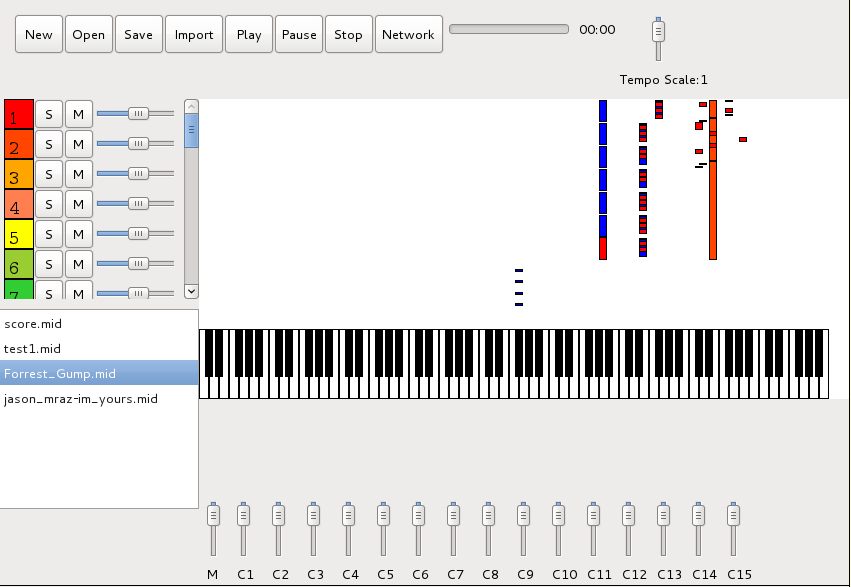
\includegraphics[width=0.75\linewidth]{2/1.png}}
\caption{HCMP Player GUI Screenshot}
\end{figure}

\section{Layout}
Figure 2.2 is a layout of the GUI of the HCMP Player. We use absolute position layout 
to arrange each component. The whole area 
covers 800 * 600 pixels. The top part is the menu panel 800 * 200 pixels 
in size. The track panel and 
the library panel share the middle-left part, each is 200 * 200 pixels in size. 
The middle-right part is 400 * 600 pixels in size, holding a MIDI keyboard and data 
display component. The bottom part is the channel panel. The container is subclass of
Window class, which works as a window to bound every object inside this area. 

\begin{figure}[H]
\center{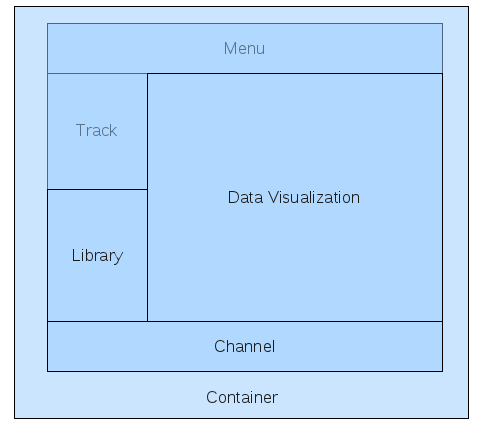
\includegraphics[width=0.6\linewidth]{2/5.png}}
\caption{HCMP Player Layout}
\end{figure}

\section{GUI Component}

\subsection{Menu Panel}

Figure 2.3 is a screenshot of the menu panel. The menu panel integrates most of the control 
functions for the HCMP Player. New, open and save buttons form a group. The group is used to 
operate the configuration file. The configuration file offers a way to save parameters for a
future session. Play, pause and stop buttons form another group. 
this group is used to directly control playback from the HCMP Player.
The network button is for the HCMP Player  
network function, after clicking the button, the player will automatically 
initiate a connection to a remote server, the IP address and port number pair is 
predefined in the configuration file and can be easily modified. Once the connection is 
successfully built, all controls will be transferred to the remote server. 
The network function will be explained in more detail in following
chapters. The menu panel also contains a slider to change 
tempo. The slider indicates of tempo scale factor. For example, 
if the original tempo is 90 BMP, and the slider is set to scale factor 1.5, 
the tempo will be 1.5 * 90 
BMP when playing the file. The import button is used to import a MIDI file 
into the HCMP Player. Once a MIDI file is successfully imported into the HCMP Player  
, the track panel, library panel and data display component will be updated.
The track path will also be recorded into the configuration file, so that the user 
will not need to import the same file again.

\begin{figure}[H]
\center{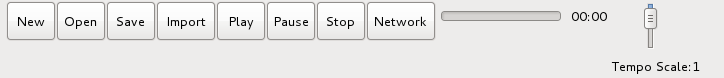
\includegraphics[width=0.8\linewidth]{2/6.png}}
\caption{HCMP Player Menu Panel}
\end{figure}

\subsection{Track Panel}

Figure 2.4 is a screenshot of the track panel. The track panel is used to 
control each track's parameters, volume, solo, mute etc. The color
block at the front of panel indicates its color in the data display component . The 
track panel will be automatically populated once a MIDI file is successfully 
loaded into the HCMP Player.
\begin{figure}[H]
\center{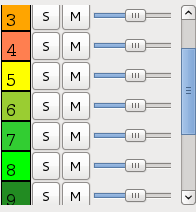
\includegraphics[width=0.3\linewidth]{2/7.png}}
\caption{HCMP Player Track Panel}
\end{figure}

\subsection{MIDI Keyboard and Data Display}
Figure 2.5 is a screenshot of the data display component. It is made up of a virtual  
keyboard and a MIDI note canvas. After successfully loading a MIDI file, the MIDI 
note canvas will 
draw each MIDI note in this area. When playing a MIDI file, the MIDI canvas will 
automatically update the position of each MIDI note. 

The virtual keyboard has 9 octaves and 108 keys. Both the white and black keys 
are drawn by the canvas. Every MIDI note will be highlighted in the 
virtual MIDI keyboard, based on its pitch, while playing. The canvas update speed is 
coordinated with the player engine so that the display and MIDI 
output are synchronized. This avoids asynchronized speed 
of canvas update and playing MIDI note problems. The Player engine is responsible for 
updating the beat, and it 
periodically sends synchronization information to the GUI. After receiving updated 
information from the player engine, the GUI will update all MIDI notes in the canvas by 
redrawing the whole canvas.

Each color of the MIDI note represents a track inside 
a MIDI file. In the current version, the color for each track's MIDI note is 
predefined. MIDI canvas scroll speed is linear to the tempo of MIDI. Whenever 
a user makes a change to the tempo, the scroll speed of the MIDI canvas will adjust
accordingly. When a user mutes a
track, its color MIDI note in MIDI canvas will temporarily be set to invisible. 
The canvas
update frequency is 20Hz. To make logic easier, every time an update event 
happens, the whole MIDI canvas will be redrawn. The MIDI canvas is 400 * 600 pixels
in size, and these pixels are updated 20 times every second. The Chapter 6, we will
discuss the performance issue of the canvas update implementation. A test case is
designed to evaluate the general performance of this object. There is a canvas 
buffer data structure to store all the ``visible'' MIDI notes inside data 
display object. Usually, the size of a MIDI file is no more than 10MB. To improve
the general efficiency of canvas, a cache like data structure is set in 
every canvas object. Based on the test case of the Chapter 6, there is no
significant lagging in display and the overall performance of using redraw 
method is acceptable.

\begin{figure}[H]
\center{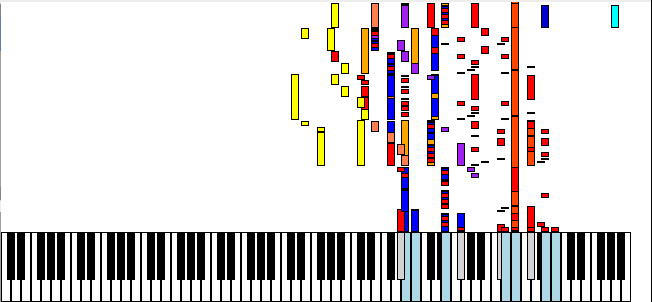
\includegraphics[width=0.7\linewidth]{2/3.png}}
\caption{HCMP Player Data Display Component}
\end{figure}

\subsection{HCMP Player Library}

Figure 2.6 is a screenshot of the MIDI library panel. This simple MIDI library is 
used to retain all the MIDI files that have ever been successfully loaded into 
the HCMP Player. 
The configuration file of the HCMP Player stores all the file names and its paths, 
when the user next launches the HCMP Player, it can load
recently opened MIDI files immediately. When a user clicks any file in the library, 
the GUI looks up a hash-like data structure and fetches its file path 
(if it exists), the GUI then automatically
loads this information into the HCMP Player. If the MIDI file failed to load, 
the library and its configuration file will remove the obsolete entry, then 
update the library panel.

\begin{figure}[H]
\center{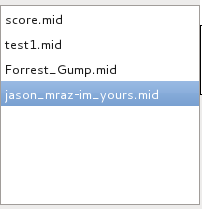
\includegraphics[width=0.3\linewidth]{2/8.png}}
\caption{HCMP Player Library Panel}
\end{figure}

\section{Player Mode}

The HCMP Player has two modes, stand-alone mode and network mode. 
In stand-alone mode, the HCMP Player can be used as a normal MIDI player. 
The user can load and play any MIDI file. In network mode, 
the HCMP Player will connect to a remote 
server. In the HCMP project, the server contains a conductor, that 
is responsible for communication and coordination with all HCMP Player instances. 
For example, 
a typical workflow for the conductor includes reading cues from external resources, 
then issuing commands to all the connected instances of the HCMP Player.

\subsection{Stand-alone Mode}

When launching the program, the HCMP player is by default in stand-alone mode, 
with the GUI component's function as described above. 
The user can use the HCMP Player to play MIDI files, change tempo, change volume, etc.


\subsection{Network Mode}

When the user clicks the network button, 
the HCMP player will enter
network mode. This mode first initiates a connection request 
to the remote server. The address and port number of the remote server is 
stored in the HCMP Player configuration file. If no reply is received within
timeout period, the HCMP player will ``rollback'' to the default stand-alone mode.
If a confirmation signal is received from the
remote server, the 2-way connection between the HCMP Player and 
remote server is successfully created allowing the HCMP Player and 
remote server to communicate. Control of the HCMP 
Player will partially be ``transferred'' to the remote server. 
In this mode, the player control buttons play, pause   
and stop continue to work as normal. To avoid conflict problems, other buttons will 
be temporarily disabled, and the binding method for these buttons is replaced by
another set of functions. The detailed network API will be explained  
in the Chapter 5.
